\renewcommand\footnoterule{}
\begin{titlepage}
    \thispagestyle{fancy}
    \setlength{\headheight}{12.0pt}
    %\lhead{Freie Universität Berlin, Institute for Computer Science}
    \renewcommand{\headrulewidth}{0pt}
    %\renewcommand{\footrulewidth}{1pt}

    \vspace*{\fill}
    \begin{center}
        \setlength{\fboxsep}{1em}
        \fbox{
            \parbox{0.75\linewidth}{
                \centering
                \textsc{
                    \Large
                    A Comprehensive Description of the\\\vspace{0.1cm}
                    Quantum HHL Algorithm and its Application\\\vspace{0.1cm}
                    in the Cryptanalysis of the AES
                }
            }
        }

        \vspace{\baselineskip}

        \vspace{\baselineskip}

        \vspace{\baselineskip}

        % See https://sites.math.washington.edu/~reu/docs/latex_symbols.pdf
        %\renewcommand{\thefootnote}{\(^\dagger\)}
        \renewcommand{\thefootnote}{\(^\text{\varhexagon}\)}
        valentinpi\footnote{E-Mail: \href{mailto:valenpi@gmx.de}{valenpi@gmx.de} - Website: \href{https://valentinpi.github.io}{valentinpi.github.io}}
        \renewcommand{\thefootnote}{\arabic{footnote}}

        Student Number: \textsc{Redacted}

        Date of Birth: \textsc{Redacted}

        \vspace{0.5cm}

        Bachelor Thesis

        Bachelor of Science

        Major in Computer Science

        \vspace{0.5cm}

        First Supervisor: \textsc{Redacted}

        Second Supervisor: \textsc{Redacted}

        Freie Universität Berlin, Institute for Computer Science

        \vspace{0.5cm}

        %Freie Universität Berlin, Institute for Computer Science

        %\vspace{0.5cm}

        Date of Submission: January 23, 2023
    \end{center}
    \vspace*{\fill}
\end{titlepage}

%\raggedleft \large \emph{To my father and my mother.} \normalsize
%\raggedleft \large \emph{To my future wife.} \normalsize

%\newpage

\begin{adjustwidth}{2cm}{2cm}
    \begin{abstract}
        \noindent Systems of linear equations appear almost everywhere in the mathematical sciences. Let it be machine learning, economic simulations, geometry or even in the field of cryptography. It is commonly known, that the classical Gaussian elimination method achieves a runtime of \(\onot(N^3)\) for such a system of \(N \in \mathbb{N}_{\geq 1}\) equations and variables. The fastest known classical approximation algorithm, the so-called conjugate gradient method, yields a complexity of \(\onot(N s \sqrt{\kappa} \log_2(1/\varepsilon))\), where \(\kappa \in \mathbb{R}_{\geq 1}\) is the condition number of the matrix, \(s \in \mathbb{N}\) its sparsity and \(\varepsilon > 0\) the error cap.

        \noindent In this thesis, we will give a description and a mathematically rigorous analysis of the quantum algorithm by Harrow, Hassidim and Lloyd (HHL), which achieves an exponential speedup to a solution to this problem given several restrictions, to a runtime of about \(\tilde{\onot}(\kappa^2s^4\log_2(N)/\varepsilon)\). We further discuss its improvements and limitations. Our contribution lies in the explicit description of the smaller auxiliary algorithms involved, as well as more detailled runtime and error bounds.
        
        \noindent Lastly, we describe, how to create simple systems of equations for key recovery of AES encrypted blocks and shortly present recent results on the application of HHL for the cryptanalysis of the Advanced Encryption System (AES) block cipher.
    \end{abstract}
    
    \renewcommand{\abstractname}{Zusammenfassung}

    \begin{abstract}
        \noindent Lineare Gleichungssysteme lassen sich an fast jeder Stelle in den mathematischen Wissenschaften wiederfinden. Sei es im maschinellen Lernen, ökonomischen Simulationen, in der Geometrie oder in der Kryptographie. Es ist im Allgemeinen bekannt, dass die klassische Lösungsmethode durch Gaußsche Eliminierung eine Laufzeit von \(\onot(N^3)\) für ein System von \(N \in \mathbb{N}_{\geq 1}\) Gleichungen und Variablen besitzt. Der schnellste bekannte klassische Approximationsalgorithmus, die sogenannte Conjugate Gradient-Methode, besitzt eine Komplexi\-tät von \(\onot(N s \sqrt{\kappa} \log_2(1/\varepsilon))\), wobei \(\kappa \in \mathbb{R}_{\geq 1}\) die Konditionsnummer der Matrix, \(s \in \mathbb{N}\) die maximale Anzahl der Einträge pro Zeile und \(\varepsilon > 0\) die erlaubte Fehlerschranke ist.

        \noindent In dieser Arbeit geben wir eine Beschreibung und eine mathematisch rigorose Analyse von dem Quantenalgorithmus von Harrow, Hassidim und Lloyd (HHL), welcher für die Lösung eines linearen Gleichungssystemes eine exponentielle Beschleunigung, unter mehreren Einschränkungen, zu einer Laufzeit von etwa \(\tilde{\onot}(\kappa^2s^4\log_2(N)/\varepsilon)\) erreicht. Wir diskutieren weiterhin die Verbesserungen und Einschränkungen von dem Algorithmus. Unser Beitrag liegt in der expliziten Beschreibung der kleineren Hilfsalgorithmen, welche involviert sind, sowie detailliertere Laufzeit- und Fehlerschranken.
        
        \noindent Zuletzt beschreiben wir, wie einfache Gleichungssysteme für die Schlüsselgewinnung aus mit AES verschlüsselten Datenblöcken formuliert werden können und präsentieren außerdem kurz neue Ergebnisse in der Anwendung von HHL für die Kryptanalyse von dem Advanced Encryption System (AES) Blockchiffre.
    \end{abstract}

    \newpage

    \begin{center}
        \textbf{Selbstständigkeitserklärung}
    \end{center}

    \vspace{0.5\baselineskip}

    Ich erkläre gegenüber der Freien Universität Berlin, dass ich die vorliegende Bachelorarbeit selbstständig und ohne Benutzung anderer als der angegebenen Quellen und Hilfsmittel angefertigt habe.

    \vspace{0.5\baselineskip}

    Die vorliegende Arbeit ist frei von Plagiaten. Alle Ausführungen, die wörtlich oder inhaltlich aus anderen Schriften entnommen sind, habe ich als solche kenntlich gemacht.

    \vspace{0.5\baselineskip}

    Diese Arbeit wurde in gleicher oder ähnlicher Form noch bei keiner anderen Universität als Prüfungsleistung eingereicht.

    \vspace{\baselineskip}

    \vspace{\baselineskip}

    Datum: \rule{3cm}{0.5pt} \hfill Unterschrift: \rule{5cm}{0.5pt}

    \vspace{10\baselineskip}
\end{adjustwidth}

\newpage

\tableofcontents

\newpage

\listofalgorithms
\listoffigures
\listoftables

\section*{List of Abbreviations}

\newcommand{\notationentry}[2]{#1 & #2\\}

\begin{table}[!hbpt]
    \centering
    \begin{tabular}{p{0.2\linewidth}p{0.4\linewidth}}
        \notationentry{\textbf{Abbreviation}}{\textbf{Full Form}}
        \hline
        \notationentry{AA}{\emph{Amplitude Amplification}}
        \notationentry{AES}{\emph{Advanced Encryption Standard}}
        \notationentry{BCD}{\emph{Binary Coded Decimal}}
        \notationentry{eq.}{\emph{equation}}
        \notationentry{et al.}{\emph{and others} (Latin: et alia)}
        \notationentry{i.e.}{\emph{that is} (Latin: id est)}
        \notationentry{iff}{\emph{if and only if}}
        \notationentry{LCU}{\emph{linear combination of unitaries}}
        \notationentry{LSB}{\emph{least significant bit}}
        \notationentry{MSB}{\emph{most significant bit}}
        \notationentry{NIST}{\emph{National Institute of Standards and Technology}}
        \notationentry{poset}{\emph{partially-ordered set}}
        \notationentry{QM}{\emph{Quantum Mechanics}}
        \notationentry{s.t.}{\emph{such that}}
        \notationentry{SLE}{\emph{System of Linear Equations}}
        \notationentry{SVD}{\emph{Singular Value Decomposition}}
        \notationentry{VTAA}{\emph{Variable Time Amplitude Amplification}}
        \notationentry{wlog.}{\emph{without loss of generality}}
        \notationentry{wrt.}{\emph{with respect to}}
    \end{tabular}
\end{table}

\newpage

\section*{List of Notations}

Let \(m, n, q \in \mathbb{N}_{\geq 1}\) here, if not said otherwise. The following meanings for the symbols are used, if no other definition is specified.

\begin{table}[!hbpt]
    \begin{tabular}{p{0.15\textwidth}p{0.75\textwidth}}
        \notationentry{\textbf{Notation}}{\textbf{Explanation}}
        \hline
        \notationentry{\(\mathbb{N}, \mathbb{Z}, \mathbb{Q}, \mathbb{R}, \mathbb{C}\)}{The sets of natural, integral, rational, real and complex numbers. \(0 \in \mathbb{N}\) here.}
        \notationentry{\(M_P\)}{For \(M\) a set and \(P\) a logical predicate over \(M\), the set \(\{a \in M \mid P(a)\}\). For instance, \(\mathbb{N}_{\geq 1}\).}
        \notationentry{\(\leadsto\)}{Informal notation for an implication.}
        \notationentry{\(x \circ M\)}{If \(x \in U\) for some universe \(U\) and \(M \subseteq U\) and \(\circ\colon U \times U \mapsto U\), the set \(\{x \circ y \mid y \in M\}\)}
        \notationentry{\(\Im(f)\)}{For a function \(f\colon A \to B\) with \(A\) and \(B\) being sets, the image \(f(A)\).}
        \notationentry{\(\ker(f)\)}{For a function \(f\colon A \to \mathbb{C}\) with \(A\) being a set, the preimage of zero \(f^{-1}(0)\), i.e. the kernel.}
        \notationentry{\(\otimes\)}{\emph{Kronecker product}, the standard tensor product used here.}
        \notationentry{\(\simeq\)}{Isomorphy relation.}
        \notationentry{\(\cong\)}{Isometric isomorphy equivalence relation.}
        \notationentry{\(\hookdoubleheadrightarrow\)}{Mapped under isomorphism.}
        \notationentry{\(\overset{\cong}{\hookdoubleheadrightarrow}\)}{Mapped under isometric isomorphism.}
        \notationentry{\([a, b]_M\)}{For a poset \((M, \leq)\) and \(a, b \in M\), the set \(\{r \in M \mid a \leq r \leq b\}\).\footnote{Often used for \emph{integer intervals}.}}
        \notationentry{\(\text{id}_M\)}{For a set \(M\), the identity function \(\text{id}_M\colon M \to M, x \mapsto x\).}
        \notationentry{\(A^{\otimes n}\)}{For \(p \in \mathbb{N}_{\geq 1}\) and some \(A \in \mathbb{C}^{m \times p}\), the tensor product power \(\bigotimes_{n} A\).}
        \notationentry{\(A^*, A^t, A^\dagger\)}{For a matrix \(A \in \mathbb{C}^{m \times n}\), the associated conjugate, transposed and adjoint matrices.}
        \notationentry{\(\mathbb{F}^{m \times n}\)}{Set of matrices of format \(m \times n\) with coefficients from a field \(\mathbb{F}\).}
        \notationentry{\(\mathbb{F}_q\)}{The set \([0, q-1]_{\mathbb{N}}\) for \(q \in \mathbb{N}_{\geq 1}\).}
        \notationentry{\(\gf(p)\)}{\emph{Galois field} with \(p\) elements, where \(p \in \mathbb{N}\) is prime.}
        \notationentry{\(\delta_{ij}\)}{\emph{Kronecker delta} for \(i, j \in \mathbb{N}\). Defined as \(\delta_{ij} \coloneqq (i = j)\).}
        \notationentry{\(E_n\)}{Unit matrix of size \(n \times n\).}
        \notationentry{\(\sigma_y\)}{\emph{Pauli Y matrix} \(-i \ket{1}\bra{0} + i\ket{0}\bra{1}\) \cite[p. 168]{Griffiths2018}.}
        \notationentry{\(\ket{k}, k \in \mathbb{N}\)}{\(k\)th canonical basis vector of the Hilbert space \(\mathbb{C}^n\), where \(k < n\).}
        \notationentry{\(\rk\)}{Matrix rank.}
        \notationentry{\(\theta_{\mathcal{F}}, \theta \in \mathbb{N}\)}{\(\theta_{\mathcal{F}} \in \mathbb{R}\) is the real number represented by \(\theta\) in a floating-point-format. For instance, in IEEE-754, a fixed-point-format or BCD.}
        \notationentry{\(\ket{\lambda}, \lambda \in \mathbb{R}\)}{\(\ket{\lambda}\) denotes a canonical basis vector \(\ket{k}\) of \(\mathbb{C}^n\), \(k \in [0, n-1]_{\mathbb{N}}\), s.t. \(k_{\mathcal{F}}\) is close to \(\lambda\). When we develop a unitary, that utilizes a \(\lambda\) value, the necessary conversions are implicitely assumed to be performed.}
        \notationentry{\(R[x_1, ..., x_n]\)}{The ring of polynomials with coefficients from a ring \(R\) over the variable symbols \(x_1, ..., x_n\).}
        \notationentry{\(S^{n-1}\)}{The sphere \(\{x \in \mathbb{R}^n \mid \norm{x} = 1\}\) with the standard norm.}
        \notationentry{\(\sphericalangle(\cdot, \cdot)\)}{Angle between two vectors in a euclidian vector space \((V, \langle \cdot, \cdot \rangle)\). Defined as \(\sphericalangle(u, v) \coloneqq \arccos\left(\frac{\langle u, v \rangle}{\norm{u}\norm{v}}\right)\) for \(u, v \in V \setminus \{0\}\) with \(\norm{\cdot}\) being the associated norm.}
        \notationentry{\(\omega_N\)}{\(\omega_N \coloneqq e^{2 \pi i/N}\). Looking in a mathematically positive direction on \(S^1\), the \emph{first \(N\)th complex unit root besides \(1\)}.}
        \notationentry{\(\diag(A_1, ..., A_r)\)}{For \(A_1, \in \mathbb{F}^{m_1 \times n_1}, ..., A_r \in \mathbb{F}^{m_r \times n_r}\) for a field \(\mathbb{F}\) and \(r, m_1, n_1, ..., m_r, n_r \in \mathbb{N}_{\geq 1}\), the diagonal matrix with blocks \(A_1, ..., A_r\).}
        \notationentry{\(U^\perp\)}{For a subspace \(U \subseteq V\) of a vector space \(V\), the \emph{orthogonal complement} of \(U\).}
        \notationentry{\(\expectation[X]\)}{For a discrete finite random variable \(X\colon (\Omega, \Pr) \to \mathbb{R}\) over a discrete finite probability space \((\Omega, \Pr)\), its expectation value \(\sum_{x \in \Omega} \Pr(X = x) x\).}
        \notationentry{\(\poly(T_1, ..., T_n)\)}{With runtime terms \(T_1, ..., T_n\), for one \(p \in \mathbb{R}[x]\), which depends only on \(T_1, ..., T_n\), the class \(\onot(p)\).}
        \notationentry{\(A \leq_p B\)}{\(A\) is polynomially time reducible to \(B\), see \Cref{hardness_results}, for languages \(A, B \subseteq \Sigma^*\).}
    \end{tabular}
\end{table}

\paragraph*{Indexing of Vectors and Matrices} Vectors in \(\mathbb{F}^n\), where \(\mathbb{F}\) is a field, will always be interpreted as column vectors. Vector and matrix entries are not zero-indexed, if not said otherwise. Matrices are indexed column-first. We may also index complex numbers, since \(\mathbb{C} \cong \mathbb{R}^2\). The bra-ket notation is used for valid quantum registers, i.e. normalized vectors in Hilbert spaces and their associated functionals. Otherwise not. We never omit the bra-ket notation to index the vectors. We further use a notation for generating matrices of form \(A \coloneqq (p(i, j))_{i, j \in m \times n} \in \mathbb{F}^{m \times n}\). By that, we mean that for any \(i \in [1, m]_{\mathbb{N}}\), \(j \in [1, n]_{\mathbb{N}}\), we have \(a_{ij} = p(i, j)\), where \(p\colon [1, m]_{\mathbb{N}} \times [1, n]_{\mathbb{N}} \to \mathbb{F}\) is a function.

\paragraph*{Standard Product and Norm} We use the general definition from \cite[p. 219]{Werner2018} for standard products. The symbols \(\braket{\cdot}{\cdot}\) and \(\norm{\cdot}\) are reserved for the complex standard product and its induced norm, defined as:
\begin{align}
    \bra{u}\ket{v} \coloneqq \sum_{i=1}^n u_iv_i^* \qquad \norm{u} \coloneqq \sqrt{\langle u, u\rangle}
\end{align}
For \(\ket{u}, \ket{v} \in \mathbb{C}^n\). Furthermore, the symbol \(\norm{\cdot}\) is also reserved for the operator norm used here, see \Cref{operator_norm}.

\paragraph*{Sets and Operations} When considerung a group, ring, field, vector space or another structure, we often omit the explicit statement of the associated operations.

\paragraph*{Switching between Matrices and Tuples} Note, that by \emph{column-major} and \emph{row-major}, we refer to the order, in which the entries of a tuple or matrix are mapped to a respective matrix or tuple. For instance, we may enumerate the vector \((0, 1, 2, 3) \in \mathbb{R}^4\) in either column-major- or row-major-enumeration into a \(2 \times 2\)-matrix, yielding respectively:
\begin{align}
    \begin{pmatrix}
        0 & 2\\
        1 & 3
    \end{pmatrix} \text{ or }
    \begin{pmatrix}
        0 & 1\\
        2 & 3
    \end{pmatrix}
\end{align}

\newpage

\null
\vfill

\begin{figure*}[!hbpt]
    \centering
    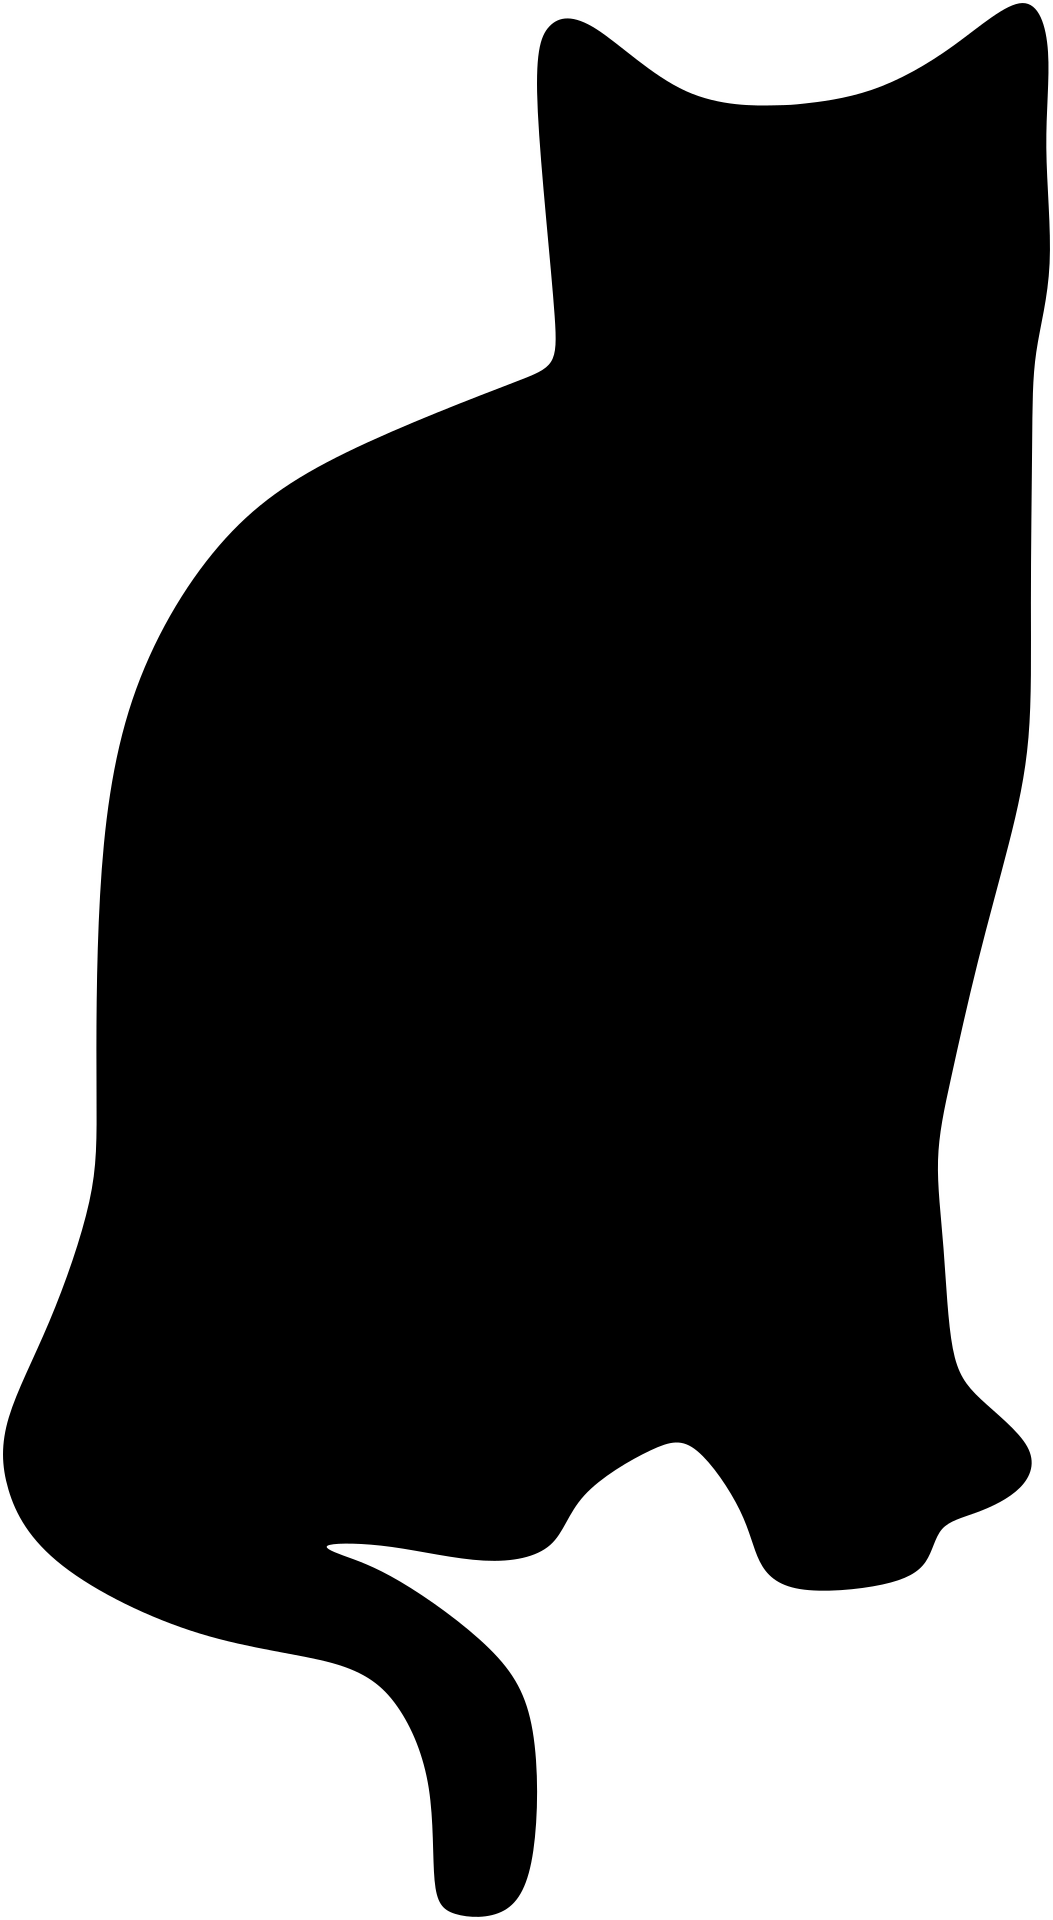
\includegraphics{img/schroedingers_cat.png}
    \caption{A famous cat. She is cute and not a sign of bad luck. She is both completely blacked out with no life sign, whilst standing upright.}
\end{figure*}

\vfill

\newpage

\phantom{}

\newpage
